\documentclass[conference]{IEEEtran}

\usepackage{graphicx}
\usepackage{booktabs}
\usepackage{amsmath}
\usepackage{url}

\graphicspath{{figures/}{../resultsAct3/}}

\begin{document}

\title{How Many Threads? Shared-Memory Parallelism and SIMD Vectorization
in Dense Matrix Multiplication}

\author{
\IEEEauthorblockN{Carlos Montesdeoca}
\IEEEauthorblockA{Big Data Course --- University of Las Palmas de Gran Canaria\\
Academic Year 2026--2027\\
Assignment 3: Parallel Matrix Multiplication}
}

\maketitle

\begin{abstract}
This study investigates how the number of threads affects the performance of a
dense $n \times n$ matrix multiplication in shared memory, and when parallel
execution is beneficial. A sequential $O(n^3)$ baseline (classic i-j-k triple
loop in C with \texttt{double} precision) is compared against an OpenMP
parallelization of the same kernel over matrix rows, using thread counts
$p \in \{1, 2, 4, 8, 16, 22, 28\}$ on a hybrid 16-core/22-thread Intel Core
Ultra 7 155H. Inputs are deterministic shared matrices up to $n = 1000$; each
configuration is measured 5 times after 2 warm-ups with a monotonic
microsecond-resolution timer, reporting medians and interquartile ranges. For
$n = 1000$, speedup grows sub-linearly and saturates at $S(p) \approx 5.45$ for
$p \geq 16$, with efficiency dropping from $1.04$ ($p=2$) to $0.25$ ($p=22$);
oversubscription ($p=28$) yields no further gain. The framework overhead of
running OpenMP with a single thread is small ($\approx 1.4\%$). As an optional
extension, a sequential i-k-j variant is evaluated under three compiler
configurations: reordering the loops alone makes the kernel vectorizable and
reduces the $n=1000$ time from $858$ ms to $288$ ms, auto-vectorization with
\texttt{-O3} reduces it further to $186$ ms, and \texttt{-march=native} reaches
$157$ ms --- comparable to the 16-thread unvectorized parallel run. Conclusions
are limited to the tested hardware, inputs and configurations.
\end{abstract}

\begin{IEEEkeywords}
matrix multiplication, OpenMP, shared-memory parallelism, speedup, SIMD
vectorization, performance evaluation
\end{IEEEkeywords}

\section{Introduction}
\label{sec:intro}

Dense matrix multiplication is the canonical workload of scientific computing
and a standard vehicle for teaching performance engineering: its $O(n^3)$
arithmetic cost and $O(n^2)$ storage make both thread-level parallelism and
data-level vectorization directly observable. Modern consumer CPUs no longer
offer homogeneous cores; they combine performance (P) and efficiency (E)
cores, hardware threads, and wide SIMD units, so the classical question
``how many threads should I use?'' no longer has a simple answer.

The motivating question of this assignment is: \textbf{how does the thread
count $p$ affect the execution time of an OpenMP parallelization of a basic
dense matrix multiplication, compared with an equivalent sequential baseline,
and where does the speedup saturate?} We additionally ask whether the
framework overhead is visible at $p=1$, whether oversubscribing the hardware
is harmful, and (as an optional extension) how much performance is available
from compiler auto-vectorization when the loop order is chosen to expose it.

The hypotheses registered before the measurements were:
\begin{itemize}
\item \textbf{H1:} Speedup will be sub-linear and will saturate well below the
22 hardware threads, because the machine is heterogeneous (only 6 P-cores) and
the kernel becomes memory-bandwidth bound at high $p$.
\item \textbf{H2:} The OpenMP runtime overhead at $p=1$ will be small
(single-digit percent) but measurable, since the parallel region adds fork and
join costs to an otherwise identical kernel.
\item \textbf{H3:} A vectorizable loop order (i-k-j) will provide a larger
single-core gain than adding threads beyond saturation, and the two techniques
are complementary.
\end{itemize}

Section~\ref{sec:bg} reviews the background; Section~\ref{sec:method}
documents the methodology; Sections~\ref{sec:results} and
\ref{sec:discussion} present and discuss the results; and
Section~\ref{sec:concl} concludes.

\section{Background}
\label{sec:bg}

\subsection{Dense matrix multiplication and loop order}
Given $\mathbf{C} = \mathbf{A}\mathbf{B}$ with square $n \times n$ matrices, the
direct algorithm computes each element as an inner product of a row of
$\mathbf{A}$ and a column of $\mathbf{B}$, requiring $2n^3$ floating-point
operations~\cite{golub2013}. The classic i-j-k triple loop accumulates the
innermost product into a single element $C_{ij}$, which is favorable for
register reuse but performs a floating-point reduction in the innermost loop.
In the i-k-j order, the innermost loop performs the rank-1 update
$C_{i,:} \mathrel{+}= A_{ik}\,\mathbf{B}_{k,:}$, i.e.\ a full row of $\mathbf{C}$
is updated with one scalar times a contiguous row of $\mathbf{B}$. Both orders
perform the same arithmetic work and use the same storage, but i-k-j exposes
data-level parallelism that a compiler can vectorize without reassociating a
reduction~\cite{hager2011}.

\subsection{OpenMP, speedup and efficiency}
OpenMP is the de-facto standard shared-memory API for C/C++/Fortran; programs
annotate loops with \texttt{\#pragma omp parallel for}, and the runtime
creates a team of $p$ threads that share memory and execute the loop body in
parallel~\cite{dagum1998,openmp52}. Given the sequential time
$T_{\text{seq}}(n)$ and the parallel time $T_p(n)$ for the same input, the
speedup and efficiency are defined as
\begin{equation}
S(p) = \frac{T_{\text{seq}}(n)}{T_p(n)}, \qquad
E(p) = \frac{S(p)}{p} \in [0, 1].
\end{equation}
Amdahl's law bounds $S(p)$ by the inverse of the serial fraction $f$,
$S(p) \leq 1/(f + (1-f)/p)$~\cite{amdahl1967}; in practice, synchronization,
load imbalance and memory bandwidth further reduce the attainable speedup,
which can be visualized with the roofline model~\cite{williams2009}.

\subsection{Auto-vectorization and hybrid CPUs}
Compilers such as GCC vectorize innermost loops at \texttt{-O3} when the loop
dependencies permit it; the report \texttt{-fopt-info-vec-optimized} provides
direct evidence of which loops were vectorized~\cite{gccopt}. Floating-point
reductions are not reassociated without \texttt{-ffast-math}, so the i-j-k
innermost loop cannot be vectorized under strict semantics, while the i-k-j
rank-1 update can. The test machine is an Intel Core Ultra 7 155H (Meteor
Lake): 6 P-cores (2 threads each), 8 E-cores and 2 low-power E-cores, 22
hardware threads in total, with P-cores boosting to 4.8~GHz and E-cores to
3.8~GHz~\cite{intel155h}. Thread placement across heterogeneous cores is
therefore a first-order effect on any scaling curve.

\section{Methodology}
\label{sec:method}

\subsection{Implementations}
All kernels are written in C, use \texttt{double} precision and store matrices
as arrays of row pointers (\texttt{double**}); they share the CSV loader,
checksum validation and memory metric of the validated Activity~1 baseline.
Table~\ref{tab:impl} summarizes the three kernels.

\begin{table}[t]
\caption{Implementations under test}
\label{tab:impl}
\centering
\begin{tabular}{@{}ll@{}}
\toprule
Method & Description \\
\midrule
Sequential & i-j-k triple loop (baseline) \\
OpenMP & same i-j-k kernel, \texttt{parallel for} over rows \\
Sequential\_ikj & i-k-j order (SIMD study only) \\
\bottomrule
\end{tabular}
\end{table}

The OpenMP kernel distributes the outer loop (rows of $\mathbf{C}$) with
\texttt{num\_threads($p$)} and \texttt{schedule(static)}. Each row of
$\mathbf{C}$ is written by exactly one thread, so the parallelization is
inherently race-free and requires no synchronization inside the kernel.
The Sequential\_ikj kernel keeps identical arithmetic and storage; only the
loop order changes, and it is used exclusively for the vectorization study
(single thread, compiler flag sweep).

\subsection{Inputs and environment}
Inputs are dense matrices with entries drawn from $U[0,1)$ by a deterministic
generator (\texttt{random.seed(42)}); the matrices for $n \in \{10, 100, 250\}$
are identical by construction to those of Activity~1, and $n \in \{500, 1000\}$
extend the same sequence. The same pair $(\mathbf{A}, \mathbf{B})$ is used for
every method and thread count of a given $n$. Table~\ref{tab:env} lists the
execution environment; the declared budgets were 5 minutes and 4 GB per
multiplication, never reached (largest observed time: 1.19 s).

\begin{table}[t]
\caption{Execution environment}
\label{tab:env}
\centering
\begin{tabular}{@{}ll@{}}
\toprule
CPU & Intel Core Ultra 7 155H (Meteor Lake) \\
Cores/threads & 6P + 8E + 2LPE = 16 cores / 22 threads \\
RAM & 32 GB, LPDDR5 \\
OS & Windows 11 (64-bit) \\
Compiler & gcc 16.2.0 (MSYS2), \texttt{-O3 -fopenmp} \\
Timer & \texttt{QueryPerformanceCounter} ($\approx$100 ns) \\
Thread counts & $p \in \{1, 2, 4, 8, 16, 22, 28\}$ \\
\bottomrule
\end{tabular}
\end{table}

\texttt{omp\_get\_wtime()} was initially used but rejected: in libgomp on
Windows it resolves only $\approx$1~ms, which quantizes the smaller sizes; the
Windows \texttt{QueryPerformanceCounter} API~\cite{msqpc} provides the needed
resolution and is monotonic.

\subsection{Measurement protocol}
Following the common protocol of the course: 2 warm-up runs are excluded from
the samples, followed by 5 measured repetitions per configuration. Only the
multiplication kernel is timed; matrix loading, allocation and checksum
computation are outside the timed region. From the 5 raw samples we report the
\emph{median} as the central statistic and the \emph{interquartile range}
(IQR) as variability. All 255 raw measurements are retained in CSV files
(columns \texttt{size, method, threads, build, repetition, time\_seconds,
memory}).

\subsection{Correctness verification}
Two independent checks were run before benchmarking: (i) the sequential result
for $n=10$ matches NumPy's \texttt{A @ B} with maximum absolute difference
$4.9 \times 10^{-7}$ (tolerance $10^{-6}$); (ii) after every OpenMP
configuration, the checksum of $\mathbf{C}$ is compared against the sequential
reference (relative tolerance $10^{-6}$), and the elementwise difference
between sequential and parallel results is exactly zero, because both kernels
perform the same operation in the same order for every element. All 40
in-run validations passed.

\subsection{Setup limitations}
Explicit thread affinity could not be enforced: libgomp~\cite{libgomp} ignores
\texttt{OMP\_PROC\_BIND}/\texttt{OMP\_PLACES} on Windows with the message
``Affinity not supported on this configuration'', so the OS scheduler placed
the workers. The memory metric is the process working set (via
\texttt{GetProcessMemoryInfo}), which includes input matrices and runtime
overhead, and is therefore used only as a coarse indicator.

\section{Results}
\label{sec:results}

\subsection{Thread scaling}
Table~\ref{tab:n1000} reports the full thread sweep for the largest tested
size, $n = 1000$ (medians of 5 repetitions; IQR in parentheses). OpenMP at
$p=1$ is 1.4\% faster than the plain sequential baseline --- the measured
framework overhead is negligible at this granularity. Speedup grows
sub-linearly: $S(4) = 3.59$, $S(8) = 4.83$, and saturates at $S(22) = 5.45$
with $E(22) = 0.25$. Oversubscription ($p = 28 > 22$ hardware threads) does
not degrade the median much ($S = 5.41$) but efficiency halves to $0.19$.

\begin{table}[t]
\caption{Thread sweep for $n = 1000$ (median time, IQR, speedup, efficiency,
median working set)}
\label{tab:n1000}
\centering
\begin{tabular}{@{}cccccc@{}}
\toprule
Config & $T_p$ (ms) & IQR (ms) & $S(p)$ & $E(p)$ & Mem (KB) \\
\midrule
Sequential & 858.2 & 31.9 & --- & --- & 31304 \\
OpenMP $p=1$ & 846.6 & 7.7 & 1.01 & 1.01 & 31304 \\
OpenMP $p=2$ & 414.4 & 8.7 & 2.07 & 1.04 & 30888 \\
OpenMP $p=4$ & 239.2 & 16.9 & 3.59 & 0.90 & 30920 \\
OpenMP $p=8$ & 177.5 & 5.4 & 4.83 & 0.60 & 30980 \\
OpenMP $p=16$ & 157.7 & 3.3 & 5.44 & 0.34 & 31108 \\
OpenMP $p=22$ & 157.4 & 5.3 & 5.45 & 0.25 & 31208 \\
OpenMP $p=28$ & 158.5 & 1.9 & 5.41 & 0.19 & 31316 \\
\bottomrule
\end{tabular}
\end{table}

Variability is small for the parallel configurations (IQR below 2\% of the
median for $n = 1000$), and the memory footprint is essentially constant
($\approx$30.5 MB, i.e.\ the three $1000 \times 1000$ double matrices
$\approx$24 MB plus runtime), growing slightly with $p$ due to per-thread
stacks. This confirms that the experiment is compute/bandwidth bound rather
than memory-capacity bound.

\begin{figure}[t]
\centering
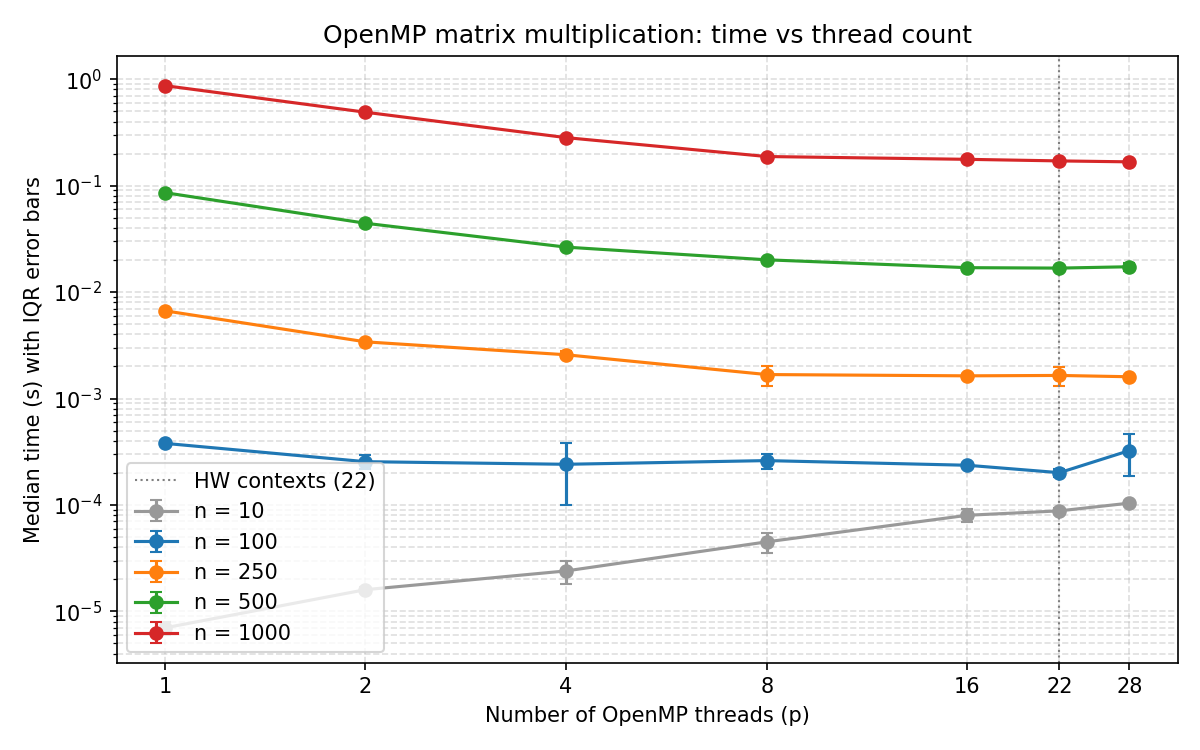
\includegraphics[width=\columnwidth]{plot_time_vs_threads_act3.png}
\caption{Median OpenMP execution time vs.\ thread count (log-log), with IQR
error bars. The dotted line marks the 22 hardware contexts. Time drops steeply
up to $p \approx 8$ and flattens afterwards; the smallest sizes are dominated
by thread management overhead and increase with $p$.}
\label{fig:time}
\end{figure}

\begin{figure}[t]
\centering
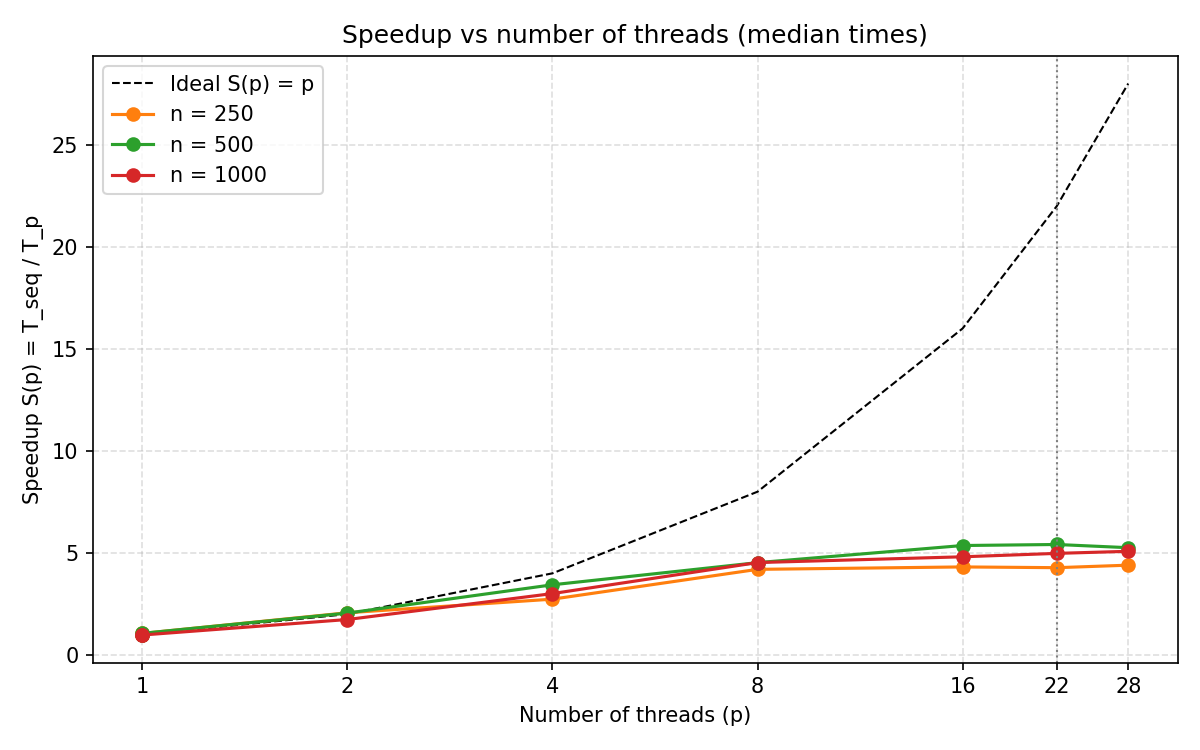
\includegraphics[width=\columnwidth]{plot_speedup_vs_threads_act3.png}
\caption{Speedup $S(p) = T_{\text{seq}}/T_p$ (median times) vs.\ thread count
for $n \in \{250, 500, 1000\}$, against the ideal line $S(p) = p$. All curves
bend away from the ideal early and saturate around $p = 16$--$22$.}
\label{fig:speedup}
\end{figure}

\begin{figure}[t]
\centering
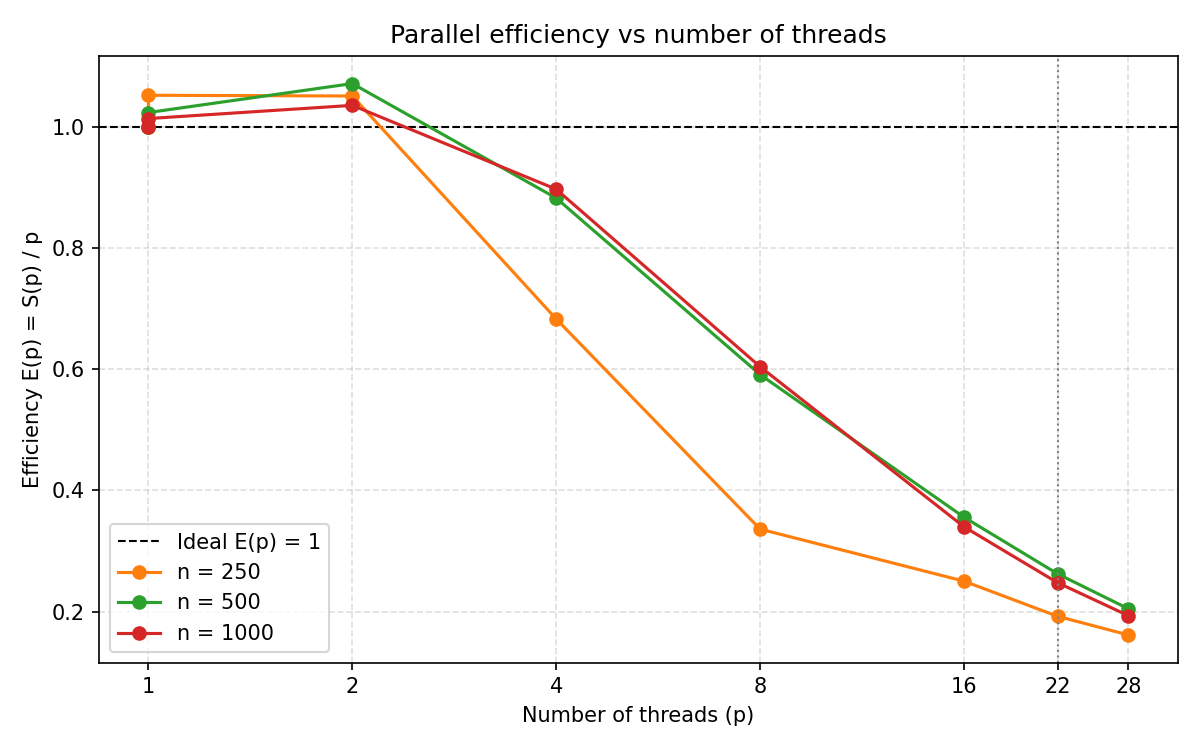
\includegraphics[width=\columnwidth]{plot_efficiency_vs_threads_act3.png}
\caption{Parallel efficiency $E(p) = S(p)/p$. Efficiency stays near 1 up to
$p = 2$--$4$ and decays roughly as $S(p)$ saturates; $p = 28$
(oversubscription) is the worst point in relative terms.}
\label{fig:eff}
\end{figure}

Figure~\ref{fig:time} shows the median time curves, and
Figs.~\ref{fig:speedup}--\ref{fig:eff} the speedup and efficiency for the three
larger sizes. The $n = 250$ curve is noisy at 1--10 ms granularity (its IQR is
a sizeable fraction of the median), so quantitative conclusions are drawn from
$n \in \{500, 1000\}$. Table~\ref{tab:cross} consolidates the speedups: larger
problems scale better (more work per unit of communication), and $n = 500$
slightly outperforms $n = 1000$ at high $p$, consistent with bandwidth sharing
across more concurrent rows.

\begin{table}[t]
\caption{Speedup $S(p)$ by problem size (median times)}
\label{tab:cross}
\centering
\begin{tabular}{@{}ccccccc@{}}
\toprule
$n$ & $p=2$ & $p=4$ & $p=8$ & $p=16$ & $p=22$ & $p=28$ \\
\midrule
250 & 2.10 & 2.73 & 2.69 & 4.01 & 4.23 & 4.52 \\
500 & 2.14 & 3.53 & 4.73 & 5.70 & 5.77 & 5.73 \\
1000 & 2.07 & 3.59 & 4.83 & 5.44 & 5.45 & 5.41 \\
\bottomrule
\end{tabular}
\end{table}

\begin{figure}[t]
\centering
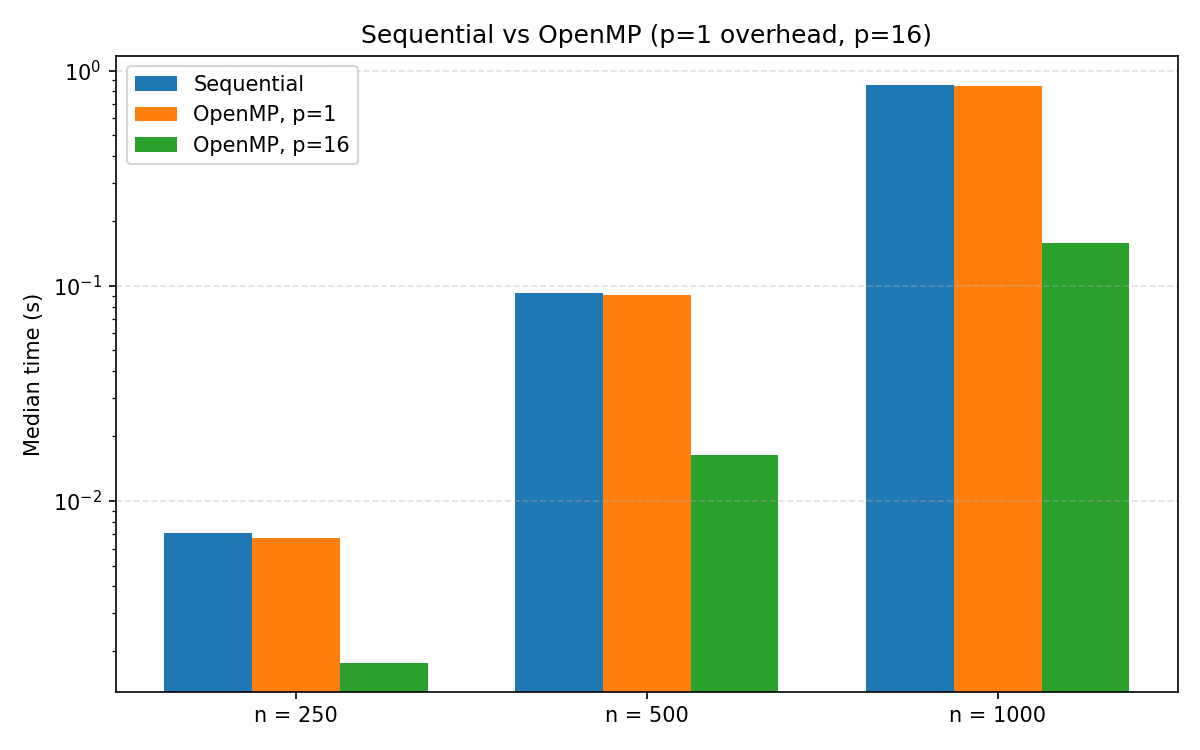
\includegraphics[width=\columnwidth]{plot_seq_vs_omp_act3.png}
\caption{Median time comparison at $n \in \{250, 500, 1000\}$: sequential
baseline, OpenMP with $p=1$ (framework overhead) and OpenMP with $p=16$
(log scale).}
\label{fig:bar}
\end{figure}

\subsection{SIMD vectorization extension}
The optional extension evaluates the Sequential\_ikj kernel under three
compiler configurations, all single-threaded, plus the i-j-k \texttt{-O3}
baseline (Table~\ref{tab:simd}). Disabling vectorization
(\texttt{-fno-tree-vectorize}) isolates the effect of the loop reorder alone:
it yields $2.98 \times$ over the i-j-k baseline at $n=1000$ purely from better
data locality. Auto-vectorization (\texttt{-O3}) then contributes a further
$1.55 \times$, and \texttt{-march=native} (AVX-512-capable Meteor Lake vector
units) another $1.19 \times$, for a total of $5.47 \times$ over the baseline
kernel.

\begin{table}[t]
\caption{SIMD study: median time (ms) of the sequential kernels, and speedup
relative to i-k-j without vectorization (last column)}
\label{tab:simd}
\centering
\begin{tabular}{@{}lcccc@{}}
\toprule
Build & $n=250$ & $n=500$ & $n=1000$ & vs.\ no-vec \\
\midrule
i-j-k, \texttt{-O3} & 7.06 & 92.90 & 858.18 & --- \\
i-k-j, \texttt{-O3 -fno-tree-vectorize} & 4.13 & 32.92 & 288.28 & $1.00\times$ \\
i-k-j, \texttt{-O3} & 2.56 & 19.81 & 186.16 & $1.55\times$ \\
i-k-j, \texttt{-O3 -march=native} & 1.80 & 14.58 & 156.85 & $1.84\times$ \\
\bottomrule
\end{tabular}
\end{table}

\begin{figure}[t]
\centering
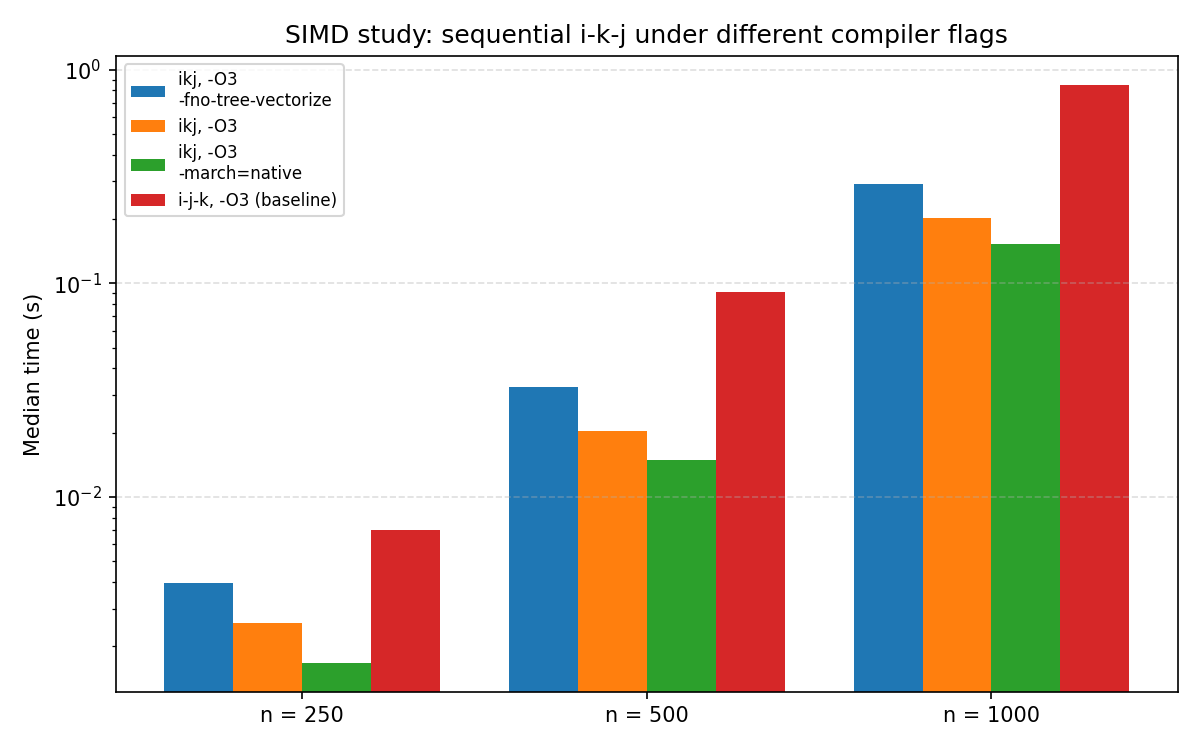
\includegraphics[width=\columnwidth]{plot_simd_act3.png}
\caption{SIMD study: median time (log scale) of the i-k-j kernel under three
compiler configurations, compared with the i-j-k \texttt{-O3} baseline, for
$n \in \{250, 500, 1000\}$.}
\label{fig:simd}
\end{figure}

Figure~\ref{fig:simd} visualizes the gap. The compiler report
(\texttt{-fopt-info-vec-optimized}) confirms that the i-k-j innermost loop is
vectorized with 16-byte vectors at \texttt{-O3}, while no vectorized loop is
reported for the i-j-k kernel, exactly as predicted by the reduction analysis.

\section{Discussion}
\label{sec:discussion}

\textbf{Answer to the research question.} On this machine and for these
inputs, threads help up to $p \approx 8$ and stop helping beyond $p \approx
16$: for $n=1000$, 8 threads deliver $S = 4.83$ ($E = 0.60$) and 22 threads
deliver only $S = 5.45$ ($E = 0.25$). The practical sweet spot is
$p \in \{8, 16\}$, where efficiency and absolute time are both reasonable.

\textbf{Why the saturation at $\approx 5.5\times$?} Three mutually compatible
explanations are supported by our data. First, the machine is heterogeneous:
only 6 P-cores exist, so a team of 16--22 threads necessarily includes slower
E-core workers, and row-partitioned work executed on an E-core inflates
$T_p$~\cite{intel155h}. Second, Amdahl's-law fitting of the observed speedups
yields an effective serial-plus-overhead fraction of $f \approx 9\%$ at $p=8$
and $f \approx 15\%$ at $p=22$: the ``serial part'' is not literal code (the
kernel has no serial section), but synchronization, scheduling and bandwidth
contention behave like one. Third, the working set of three $n=1000$ matrices
($\approx$24 MB) exceeds the 24 MB shared L3, so concurrent workers compete
for memory bandwidth, the mechanism predicted by the roofline
model~\cite{williams2009}. The fact that $n=500$ scales slightly better than
$n=1000$ at high $p$ (Table~\ref{tab:cross}) is consistent with a bandwidth
wall: more threads cannot create bandwidth.

\textbf{Overhead and superlinearity.} OpenMP at $p=1$ is within 1.4\% of the
sequential baseline (Table~\ref{tab:n1000}), so the framework fork/join cost
is negligible for kernels of this size (H2 confirmed). The mild superlinearity
at $p=2$ ($S = 2.07$, $E = 1.04$) is not evidence of ``free work'': the most
plausible cause is the frequency regime --- a single busy P-core runs at a
different point of the turbo curve than two lightly loaded cores --- combined
with median quantization. We report it as observed and do not claim a
mechanism we cannot isolate without per-core frequency counters.

\textbf{Threads vs.\ vectorization.} H3 is confirmed with a striking
cross-check: the best parallel configuration of the unvectorized i-j-k kernel
($p=16$: 157.7 ms) and the single-threaded vectorized i-k-j kernel with
\texttt{-march=native} (156.8 ms) are essentially tied. Each technique buys
roughly the same $5.5 \times$ on this workload, but they act on different
resources (cores vs.\ vector units) and are therefore complementary; combining
them (OpenMP over i-k-j) was out of scope and is the natural next experiment.
The loop reorder alone --- before any vector instruction executes ---
accounts for $3 \times$, a reminder that ``vectorizable'' often means
``cache-friendly'' at the same time.

\textbf{Threats to validity and limitations.} (i) Single machine, single
compiler, single parallelization strategy (static row partitioning, no cache
blocking); (ii) $n \leq 1000$ is modest --- larger $n$ would shift the balance
toward bandwidth even more; (iii) affinity could not be controlled on
Windows/libgomp, so thread placement is OS-dependent; (iv) the memory metric
(working set) is coarse and includes the runtime; (v) small sizes
($n \leq 250$) have measurement noise comparable to their runtime and should
not be used for scaling conclusions; (vi) frequency/turbo states were not
controlled. Conclusions are limited to the configurations actually measured.

\section{Conclusions}
\label{sec:concl}

Within the tested scope (C + OpenMP i-j-k kernel, one hybrid Intel laptop CPU,
dense inputs up to $n = 1000$), the study establishes that: (1) thread
parallelism delivers up to $5.45 \times$ speedup, saturating around
$p = 16$--$22$ with efficiency falling to $0.25$; (2) the OpenMP overhead at
$p=1$ is negligible ($\approx 1.4\%$); (3) oversubscribing the 22 hardware
threads brings no benefit; and (4) a vectorizable i-k-j ordering with
\texttt{-march=native} matches the 16-thread parallel speedup in a single
thread ($5.47 \times$ over the i-j-k baseline). What remains unresolved is how
these two axes combine (parallel i-k-j), how the curves shift on a homogeneous
server CPU or under enforced affinity, and how the saturation point moves with
$n$ far beyond the last-level cache.

\subsection*{Data and code availability}
All materials are in the GitHub repository
\url{https://github.com/CarlosMontesdeoca21/BasicMatrixMultiplication},
folder \texttt{Activity3/}: source code (\texttt{code/c/benchmark\_omp.c},
scripts in \texttt{code/python/}), raw measurements
(\texttt{data/results\_*.csv}), consolidated tables and figures
(\texttt{resultsAct3/}), and a README with the exact build and execution
commands. The matrices are regenerated deterministically (seed 42) by
\texttt{generate\_inputsAct3.py}.

\subsection*{Generative AI disclosure}
In accordance with the course policy, the author discloses the use of an AI
programming assistant (OpenCode, a large-language-model-based CLI agent) for
drafting and reviewing the C/OpenMP and Python code and for editing this
report. The student compiled, executed and validated all code, obtained all
measurements locally, generated all figures with the provided scripts, and
verified every reference cited in this paper.

\begin{thebibliography}{10}

\bibitem{amdahl1967}
G.~M. Amdahl, ``Validity of the single processor approach to achieving large
scale computing capabilities,'' in \emph{Proc. AFIPS Spring Joint Comput.
Conf.}, vol. 30, Atlantic City, NJ, USA, 1967, pp. 483--485.

\bibitem{dagum1998}
L.~Dagum and R.~Menon, ``OpenMP: An industry-standard API for shared-memory
programming,'' \emph{IEEE Comput. Sci. Eng.}, vol. 5, no. 1, pp. 46--55,
Jan.--Mar. 1998.

\bibitem{openmp52}
OpenMP Architecture Review Board, \emph{OpenMP Application Program Interface,
Version 5.2}, Nov. 2022. [Online]. Available:
\url{https://www.openmp.org/specifications/}

\bibitem{hager2011}
G.~Hager and G.~Wellein, \emph{Introduction to High Performance Scientific
Computing: A Multidisciplinary Approach}. Boca Raton, FL, USA: CRC Press,
2011.

\bibitem{williams2009}
S.~Williams, A.~Waterman, and D.~Patterson, ``Roofline: An insightful visual
performance model for multicore architectures,'' \emph{Commun. ACM}, vol. 52,
no. 4, pp. 65--76, Apr. 2009.

\bibitem{golub2013}
G.~H. Golub and C.~F. Van Loan, \emph{Matrix Computations}, 4th ed. Baltimore,
MD, USA: Johns Hopkins Univ. Press, 2013.

\bibitem{intel155h}
Intel Corp., ``Intel Core Ultra 7 Processor 155H (24M Cache, up to 4.80 GHz),''
product specifications (ARK). [Online]. Available:
\url{https://www.intel.com/content/www/us/en/products/sku/236847/intel-core-ultra-7-processor-155h-24m-cache-up-to-4-80-ghz/specifications.html}

\bibitem{msqpc}
Microsoft Corp., ``QueryPerformanceCounter function (profileapi.h),'' Microsoft
Learn. [Online]. Available:
\url{https://learn.microsoft.com/en-us/windows/win32/api/profileapi/nf-profileapi-queryperformancecounter}

\bibitem{gccopt}
Free Software Foundation, ``GCC documentation: Optimize options.'' [Online].
Available: \url{https://gcc.gnu.org/onlinedocs/gcc/Optimize-Options.html}

\bibitem{libgomp}
Free Software Foundation, ``GNU Offloading and Multi Processing Runtime
Library (libgomp), manual.'' [Online]. Available:
\url{https://gcc.gnu.org/onlinedocs/libgomp/}

\end{thebibliography}

\end{document}
